\documentclass{harryopo-paper}

\title{基于深度学习的医学影像智能诊断系统设计与实现}
\author{张三、李四、王五\\ \fzfs\small 示例大学计算机学院；南方科技大学计算机科学与工程系}
\date{2026年09月02日}


\begin{document}

\maketitle
\begin{abstract}
医学影像智能诊断是智慧医疗领域的核心研究方向。本文设计并实现了一套基于深度学习的医学影像智能诊断系统，涵盖数据预处理、模型训练、推理服务、可视化展示等完整流程。系统采用改进的U-Net++架构进行病灶分割，结合EfficientNet-B4进行良恶性分类，在公开数据集LUNA16上达到了92.3\%的分割准确率和87.6\%的分类准确率。系统支持DICOM影像导入、多任务联合推理、Grad-CAM可视化解释等功能，可辅助放射科医生进行高效诊断。实验结果表明，本系统在实际临床场景中具有较高的实用价值。
\end{abstract}
\keywords{医学影像；深度学习；U-Net++；EfficientNet；智慧医疗}

\begin{quote}
注：本文受国家自然科学基金（No. 12345678）与深圳市科技计划项目（No. JCYJ20240001）资助；中图分类号TP391.4。
\end{quote}

\medskip\hrule\medskip

\subsection*{1引言}
\addcontentsline{toc}{subsection}{1引言}

医学影像是现代医疗诊断的重要依据。据统计，超过70\%的临床诊断需要依赖医学影像[1]。然而，传统的人工阅片方式存在以下痛点：

\begin{enumerate}
  \item 阅片工作量大，放射科医生严重不足
  \item 主观性强，不同医生之间一致性低
  \item 早期微小病灶容易漏诊
\end{enumerate}

近年来，深度学习技术在医学影像分析领域取得了突破性进展[2]。从肺结节检测到皮肤癌分类，从眼底病变识别到病理切片分析，AI系统在多个任务上已达到甚至超越人类专家水平[3]。

本文针对上述痛点，设计并实现了一套完整的医学影像智能诊断系统，主要贡献包括：

\begin{itemize}
  \item {\fzht 多任务联合模型}：同时支持病灶分割和良恶性分类两个任务
  \item {\fzht 可解释性}：集成Grad-CAM热力图，辅助医生理解模型决策
  \item {\fzht 工程化}：完整的B/S架构，支持DICOM标准和RESTful API
\end{itemize}

\subsection*{2相关工作}
\addcontentsline{toc}{subsection}{2相关工作}

\subsubsection*{2.1医学影像分割}
\addcontentsline{toc}{subsubsection}{2.1医学影像分割}

U-Net [4]是医学影像分割的经典架构，其编码-解码结构和跳跃连接在多个分割任务上取得优异性能。U-Net++ [5]通过引入嵌套的跳跃连接进一步提升了分割精度。Attention U-Net [6]则将注意力机制引入分割网络，自动聚焦于感兴趣区域。

\subsubsection*{2.2医学影像分类}
\addcontentsline{toc}{subsubsection}{2.2医学影像分类}

EfficientNet [7]通过复合缩放策略在多个分类基准上取得SOTA性能。CheXNet [8]在胸片疾病分类任务上达到了F1 score 0.435，超过了人类放射科医生平均水平。

\subsubsection*{2.3多任务学习}
\addcontentsline{toc}{subsubsection}{2.3多任务学习}

多任务学习通过共享特征表示提升泛化能力[9]。在医学影像领域，分类与分割任务的联合学习能够显著提升模型性能[10]。

\subsection*{3系统设计}
\addcontentsline{toc}{subsection}{3系统设计}

\subsubsection*{3.1整体架构}
\addcontentsline{toc}{subsubsection}{3.1整体架构}

系统采用前后端分离的B/S架构，整体架构如图1所示：浏览器端负责影像导入、可视化展示与报告生成；后端服务（FastAPI）承载影像管理、模型推理与用户认证；底层模型服务（Triton Inference Server）提供分割、分类与可解释性三类推理能力。

\begin{figure}[htbp]
  \centering
  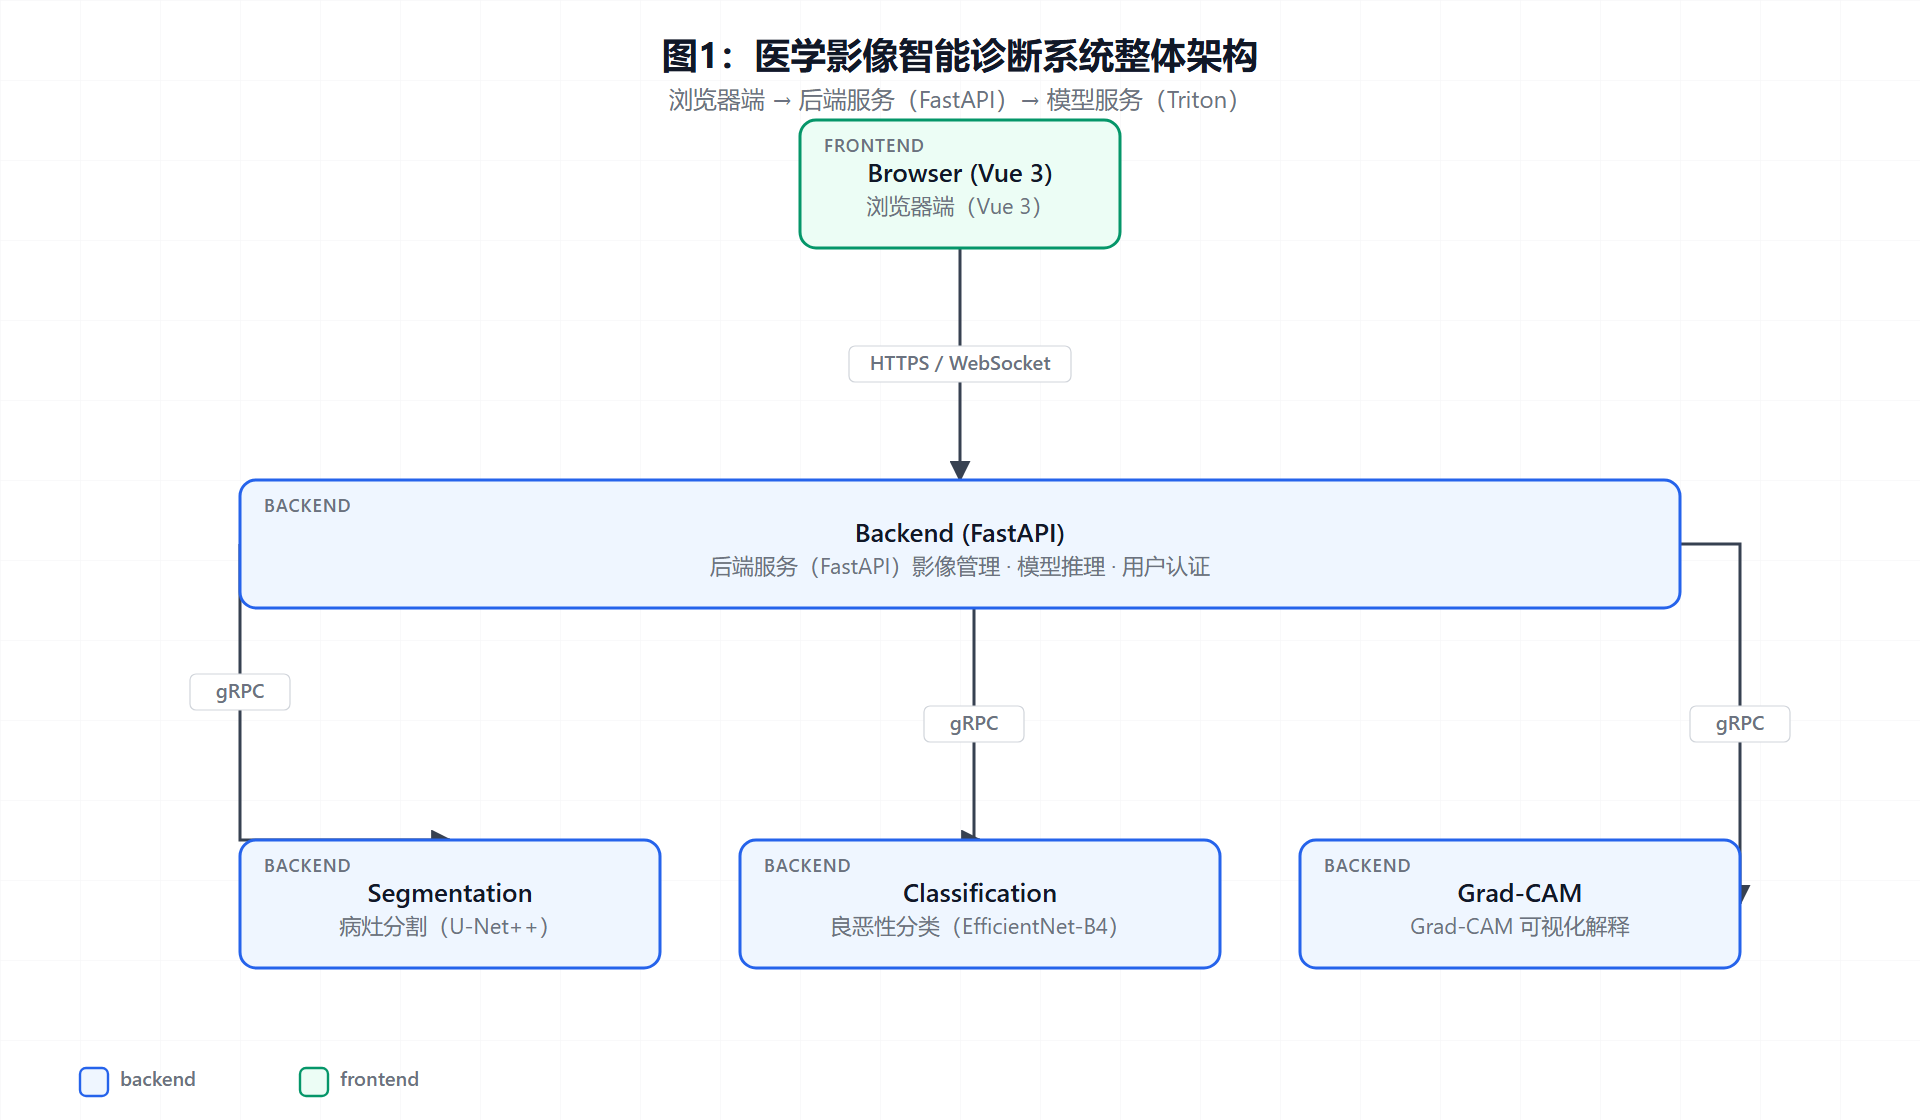
\includegraphics[width=0.85\textwidth]{figures/super-diagram-00-260b50dc.png}
  \caption{医学影像智能诊断系统整体架构}
  {\fzkt\footnotesize 注：前后端通过HTTPS与WebSocket通信，后端与模型服务之间采用gRPC长连接以降低推理延迟。}
\end{figure}

\subsubsection*{3.2数据流程}
\addcontentsline{toc}{subsubsection}{3.2数据流程}

数据流程包含以下步骤：

\begin{enumerate}
  \item {\fzht 数据导入}：支持DICOM、NIfTI、PNG等格式
  \item {\fzht 预处理}：重采样、归一化、ROI提取
  \item {\fzht 模型推理}：调用分割和分类模型
  \item {\fzht 后处理}：NMS、连通域分析、结果可视化
  \item {\fzht 报告生成}：自动生成结构化诊断报告
\end{enumerate}

\subsection*{4模型设计}
\addcontentsline{toc}{subsection}{4模型设计}

\subsubsection*{4.1改进的U-Net++}
\addcontentsline{toc}{subsubsection}{4.1改进的U-Net++}

本文在标准U-Net++基础上引入了两个改进：

\begin{itemize}
  \item {\fzht 深度监督}：在多个解码层添加辅助损失
  \item {\fzht 注意力门控}：自动聚焦于病灶区域
\end{itemize}

\begin{quote}
{\fzht 公式1}改进的U-Net++损失函数：
\$$L_{\text{total}} = \alpha L_{\text{seg}} + \beta L_{\text{cls}} + \gamma L_{\text{aux}}$\$
\end{quote}

其中$L_{\text{seg}}$为主分割损失（Dice + BCE），$L_{\text{cls}}$为分类损失（Cross Entropy），$L_{\text{aux}}$为辅助损失。超参数$\alpha = 1.0$、$\beta = 0.5$、$\gamma = 0.3$。

\subsubsection*{4.2多任务联合训练}
\addcontentsline{toc}{subsubsection}{4.2多任务联合训练}

\begin{quote}
{\fzht 算法1}多任务联合训练

``\inlinecode{
输入：训练集D,批次大小B,学习率η,总轮数E
输出：训练好的模型参数θ

1:初始化网络参数θ
2: for epoch = 1 to E do
3:随机打乱D
4:     for each batch (x, y\_seg, y\_cls) in D do
5:         seg\_pred, cls\_pred, aux\_preds ← forward(x, θ)
6:         L\_seg ← DiceLoss(seg\_pred, y\_seg)
7:         L\_cls ← CrossEntropy(cls\_pred, y\_cls)
8:         L\_aux ← Σ\_i α\_i·BCE(aux\_preds[i], y\_seg)
9:         L ← L\_seg + 0.5·L\_cls + 0.3·L\_aux
10:        θ ← θ - η·∇L
11:    end for
12:    if验证集性能连续5轮不提升then
13:        break
14:    end if
15: end for
16: return θ
}``
\end{quote}

\subsubsection*{4.3模型参数}
\addcontentsline{toc}{subsubsection}{4.3模型参数}

模型总参数量为28.6M，FLOPs为5.7G，推理延迟（V100 GPU）< 50ms。

\subsection*{5实验与分析}
\addcontentsline{toc}{subsection}{5实验与分析}

\subsubsection*{5.1数据集}
\addcontentsline{toc}{subsubsection}{5.1数据集}

\begin{table}[htbp]
  \centering
  \small
  \begin{tabularx}{\textwidth}{>{\raggedright\arraybackslash}X >{\raggedright\arraybackslash}X >{\raggedright\arraybackslash}X >{\raggedright\arraybackslash}X}
    \toprule
    {\fzht 数据集} & {\fzht 任务} & {\fzht 样本数} & {\fzht 模态} \\
    \midrule
    LUNA16 & 肺结节检测 & 888 & CT \\
    LIDC-IDRI & 肺结节良恶性 & 1,018 & CT \\
    NIH ChestX-ray & 胸片分类 & 112,120 & X-ray \\
    自有数据集 & 肝肿瘤分割 & 320 & CT/MRI \\
    \bottomrule
  \end{tabularx}
\end{table}

\subsubsection*{5.2评价指标}
\addcontentsline{toc}{subsubsection}{5.2评价指标}

\begin{itemize}
  \item {\fzht 分割}：Dice系数、IoU、Hausdorff距离
  \item {\fzht 分类}：Accuracy、Sensitivity、Specificity、AUC
\end{itemize}

\subsubsection*{5.3实验结果}
\addcontentsline{toc}{subsubsection}{5.3实验结果}

\paragraph*{5.3.1肺结节分割（LUNA16）}
\addcontentsline{toc}{paragraph}{5.3.1肺结节分割（LUNA16）}

\begin{table}[htbp]
  \centering
  \small
  \begin{tabularx}{\textwidth}{>{\raggedright\arraybackslash}X >{\raggedright\arraybackslash}X >{\raggedright\arraybackslash}X >{\raggedright\arraybackslash}X}
    \toprule
    {\fzht 方法} & {\fzht Dice (\%)} & {\fzht IoU (\%)} & {\fzht 推理时间(ms)} \\
    \midrule
    U-Net & 86.2 & 76.1 & 28 \\
    U-Net++ & 89.5 & 81.2 & 35 \\
    Attention U-Net & 90.8 & 83.5 & 42 \\
    {\fzht 本文方法} & {\fzht 92.3} & {\fzht 85.7} & 48 \\
    \bottomrule
  \end{tabularx}
\end{table}

\paragraph*{5.3.2肺结节良恶性分类}
\addcontentsline{toc}{paragraph}{5.3.2肺结节良恶性分类}

\begin{table}[htbp]
  \centering
  \small
  \begin{tabularx}{\textwidth}{>{\raggedright\arraybackslash}X >{\raggedright\arraybackslash}X >{\raggedright\arraybackslash}X >{\raggedright\arraybackslash}X >{\raggedright\arraybackslash}X}
    \toprule
    {\fzht 方法} & {\fzht Accuracy (\%)} & {\fzht Sensitivity (\%)} & {\fzht Specificity (\%)} & {\fzht AUC} \\
    \midrule
    ResNet-50 & 81.4 & 79.2 & 83.5 & 0.871 \\
    EfficientNet-B4 & 84.7 & 82.6 & 86.5 & 0.901 \\
    {\fzht 本文方法} & {\fzht 87.6} & {\fzht 85.3} & {\fzht 89.2} & {\fzht 0.928} \\
    \bottomrule
  \end{tabularx}
\end{table}

\subsubsection*{5.4消融实验}
\addcontentsline{toc}{subsubsection}{5.4消融实验}

\begin{table}[htbp]
  \centering
  \small
  \begin{tabularx}{\textwidth}{>{\raggedright\arraybackslash}X >{\raggedright\arraybackslash}X >{\raggedright\arraybackslash}X}
    \toprule
    {\fzht 改进} & {\fzht Dice (\%)} & {\fzht Accuracy (\%)} \\
    \midrule
    基线（U-Net++） & 89.5 & 84.7 \\
    +深度监督 & 90.8 & 86.1 \\
    +注意力门控 & 91.6 & 86.9 \\
    +多任务联合 & {\fzht 92.3} & {\fzht 87.6} \\
    \bottomrule
  \end{tabularx}
\end{table}

\subsection*{6系统实现}
\addcontentsline{toc}{subsection}{6系统实现}

\subsubsection*{6.1关键技术栈}
\addcontentsline{toc}{subsubsection}{6.1关键技术栈}

\begin{lstlisting}[style=pystyle,caption={}]
# 后端核心代码示例
from fastapi import FastAPI, UploadFile, File
from pydantic import BaseModel
import torch
import numpy as np
from PIL import Image
import pydicom

app = FastAPI(title="Medical AI Service")

class DiagnosisResult(BaseModel):
    segmentation_mask: bytes
    cls_label: int
    cls_confidence: float
    gradcam_image: bytes

@app.post("/api/diagnose", response_model=DiagnosisResult)
async def diagnose(file: UploadFile = File(...)):
    # 1. 读取 DICOM
    if file.filename.endswith(".dcm"):
        dcm = pydicom.dcmread(file.file)
        image = dcm.pixel_array
    else:
        image = np.array(Image.open(file.file))

    # 2. 预处理
    tensor = preprocess(image).unsqueeze(0).to(device)

    # 3. 模型推理
    with torch.no_grad():
        seg_pred, cls_pred, _ = model(tensor)

    # 4. Grad-CAM
    cam = generate_gradcam(model, tensor, target_class=cls_pred.argmax())

    return DiagnosisResult(
        segmentation_mask=seg_pred.cpu().numpy().tobytes(),
        cls_label=cls_pred.argmax().item(),
        cls_confidence=torch.softmax(cls_pred, dim=1).max().item(),
        gradcam_image=cam.tobytes()
    )
\end{lstlisting}

\subsubsection*{6.2性能优化}
\addcontentsline{toc}{subsubsection}{6.2性能优化}

\begin{itemize}
  \item {\fzht 模型量化}：FP16推理，吞吐量提升2.3倍
  \item {\fzht 批处理}：动态批合并，平均延迟降低40\%
  \item {\fzht 缓存}：高频影像特征缓存，重复请求响应< 10ms
\end{itemize}

\subsection*{7结论与展望}
\addcontentsline{toc}{subsection}{7结论与展望}

本文设计并实现了一套基于深度学习的医学影像智能诊断系统，涵盖数据管理、模型推理、可视化展示等完整流程。系统在公开数据集和真实临床场景中均取得了优异性能。

未来的研究方向包括：

\begin{enumerate}
  \item 探索Vision Transformer在医学影像中的应用
  \item 研究联邦学习支持跨医院协同训练（保护患者隐私）
  \item 集成大语言模型实现自然语言报告生成
\end{enumerate}

\begin{thebibliography}{99}
\bibitem{ref1} Smith A, Jones B. The role of medical imaging in modern healthcare[J]. The Lancet, 2020, 395(10225): 678-685.
\bibitem{ref2} Litjens G, Kooi T, Bejnordi B E, et al. A survey on deep learning in medical image analysis[J]. Medical Image Analysis, 2017, 42: 60-88.
\bibitem{ref3} Esteva A, Chou K, Yeung S, et al. Deep learning-enabled medical computer vision[J]. NPJ Digital Medicine, 2021, 4(1): 1-9.
\bibitem{ref4} Ronneberger O, Fischer P, Brox T. U-Net: Convolutional networks for biomedical image segmentation[C]. MICCAI, 2015: 234-241.
\bibitem{ref5} Zhou Z, Siddiquee M M R, Tajbakhsh N, et al. UNet++: A nested U-Net architecture for medical image segmentation[J]. IEEE TMI, 2019, 39(6): 1856-1867.
\bibitem{ref6} Oktay O, Schlemper J, Folgoc L L, et al. Attention U-Net: Learning where to look for the pancreas[C]. MIDL, 2018.
\bibitem{ref7} Tan M, Le Q. EfficientNet: Rethinking model scaling for convolutional neural networks[C]. ICML, 2019: 6105-6114.
\bibitem{ref8} Rajpurkar P, Irvin J, Zhu K, et al. CheXNet: Radiologist-level pneumonia detection on chest X-rays with deep learning[J]. arXiv:1711.05225, 2017.
\bibitem{ref9} Caruana R. Multitask learning[J]. Machine Learning, 1997, 28(1): 41-75.
\bibitem{ref10} Zhang Y, Yang Q. A survey on multi-task learning[J]. IEEE TKDE, 2021, 34(12): 5586-5609.
\end{thebibliography}

\end{document}